\begin{center}
    {\large \textbf{PHẦN I. LÝ THUYẾT XÁC SUẤT}}\\[0.3em]
    {\normalsize \textit{(Probability Theory)}}\\[1em]
    {\LARGE \textbf{CHƯƠNG 3. CÁC QUY LUẬT PHÂN PHỐI XÁC SUẤT THÔNG DỤNG}}
\end{center}

\vspace{1em}
\hrule
\vspace{1.5em}

\section{Phân phối Siêu bội (Hypergeometric Distribution)}

\subsection{Định nghĩa phân phối Siêu bội}

\begin{dinhnghia}
Xét một tập hợp gồm $N$ phần tử, trong đó có $N_A$ phần tử mang tính chất $A$ và $N - N_A$ phần tử không mang tính chất $A$ (ký hiệu là $\overline{A}$). Từ tập hợp đó, ta chọn ngẫu nhiên không hoàn lại ra $n$ phần tử ($n \le N$).

Gọi $X$ là số phần tử có tính chất $A$ lẫn trong $n$ phần tử đã chọn. Khi đó, $X$ là biến ngẫu nhiên rời rạc có \textbf{phân phối Siêu bội} (Hypergeometric distribution) với 3 tham số $N, N_A, n$.

Ký hiệu là:
\[
X \in H(N, N_A, n) \quad \text{hay} \quad X \sim H(N, N_A, n).
\]
\end{dinhnghia}

\begin{center}
\begin{tikzpicture}[scale=0.95]
    % Outer rectangle: N elements
    \draw[thick, fill=yellow!15] (-4.5,-2.3) rectangle (4.5,2.3);
    \node[above right, red!80!black] at (-4.3, 1.7) {\textbf{Tập hợp $N$ phần tử}};
    
    % Left region: NA elements with property A
    \draw[thick, fill=red!20] (-1.2,0) ellipse (2.6cm and 1.8cm);
    \node[red!80!black] at (-2.2, 0.9) {\large $N_A$ (tính chất $A$)};
    \node[blue!80!black] at (2.4, 1.2) {\large $N - N_A$ (tính chất $\overline{A}$)};
    
    % Selection: n elements
    \draw[very thick, fill=cyan!25, fill opacity=0.55] (0.8,-0.1) ellipse (2cm and 1.3cm);
    \node[above, font=\bfseries] at (1.8, -0.1) {$n$ phần tử chọn ra};
    
    % Intersection: k elements with property A
    \node[font=\bfseries, red!80!black] at (-0.2, -0.1) {$k$};
    \node[below, font=\scriptsize, align=center] at (-0.2, -0.5) {có tính chất $A$};
    
    % Outside intersection: n - k elements
    \node[font=\bfseries, blue!80!black] at (1.7, -0.5) {$n - k$};
    \node[below, font=\scriptsize, align=center] at (1.7, -0.9) {không có $A$};
\end{tikzpicture}
\end{center}

\paragraph{Miền giá trị của $X$:}
Số phần tử $k$ mang tính chất $A$ được chọn ra phải thỏa mãn:
\[
\max\{0; n - (N - N_A)\} \le k \le \min\{n; N_A\}.
\]

\paragraph{Công thức tính xác suất:}
Xác suất trong $n$ phần tử chọn ra có đúng $k$ phần tử mang tính chất $A$ là:
\[
p_k = P(X = k) = \frac{C_{N_A}^k C_{N - N_A}^{n - k}}{C_N^n},
\]
trong đó: $0 \le k \le n$ và $n - (N - N_A) \le k \le N_A$.

\begin{proof}[Chứng minh]
\begin{itemize}
    \item Số cách chọn ngẫu nhiên không hoàn lại $n$ phần tử từ tập $N$ phần tử là số tổ hợp chập $n$ của $N$: $C_N^n$ (số phần tử của không gian mẫu $|\Omega| = C_N^n$).
    \item Để chọn được đúng $k$ phần tử có tính chất $A$, ta thực hiện hai công đoạn độc lập:
    \begin{itemize}
        \item Chọn $k$ phần tử từ $N_A$ phần tử có tính chất $A$: có $C_{N_A}^k$ cách.
        \item Chọn $n - k$ phần tử còn lại từ $N - N_A$ phần tử không có tính chất $A$: có $C_{N - N_A}^{n - k}$ cách.
    \end{itemize}
    \item Theo quy tắc nhân, số kết quả thuận lợi cho biến cố $\{X = k\}$ là $C_{N_A}^k C_{N - N_A}^{n - k}$.
    \item Theo định nghĩa xác suất cổ điển, ta có điều phải chứng minh:
    \[
    p_k = P(X = k) = \frac{C_{N_A}^k C_{N - N_A}^{n - k}}{C_N^n}.
    \]
\end{itemize}
\end{proof}

\begin{vidu}[VD 1]
Một hộp phấn gồm 10 viên, trong đó có 6 viên màu trắng. Lấy ngẫu nhiên 3 viên phấn từ hộp này. Gọi $X$ là số viên phấn trắng lấy được. Lập bảng phân phối xác suất của $X$?

\paragraph{Giải.}
Ta có: $N = 10$, $N_A = 6$, $n = 3$. Vì chọn không hoàn lại nên $X \in H(10, 6, 3)$.

Miền giá trị của $X$: Do $\max\{0; 3 - 4\} = 0 \le k \le \min\{3; 6\} = 3$ nên $X \in \{0; 1; 2; 3\}$.

Các xác suất tương ứng:
\begin{align*}
P(X = 0) &= \frac{C_6^0 C_4^3}{C_{10}^3} = \frac{1 \times 4}{120} = \frac{4}{120} = \frac{1}{30} \approx 0{,}0333, \\
P(X = 1) &= \frac{C_6^1 C_4^2}{C_{10}^3} = \frac{6 \times 6}{120} = \frac{36}{120} = \frac{3}{10} = 0{,}3, \\
P(X = 2) &= \frac{C_6^2 C_4^1}{C_{10}^3} = \frac{15 \times 4}{120} = \frac{60}{120} = \frac{1}{2} = 0{,}5, \\
P(X = 3) &= \frac{C_6^3 C_4^0}{C_{10}^3} = \frac{20 \times 1}{120} = \frac{20}{120} = \frac{1}{6} \approx 0{,}1667.
\end{align*}

Bảng phân phối xác suất của $X$:
\begin{center}
\renewcommand{\arraystretch}{1.5}
\begin{tabular}{|c|c|c|c|c|}
\hline
$X$ & $0$ & $1$ & $2$ & $3$ \\
\hline
$P$ & $\dfrac{C_6^0 C_4^3}{C_{10}^3} = \dfrac{4}{120}$ & $\dfrac{C_6^1 C_4^2}{C_{10}^3} = \dfrac{36}{120}$ & $\dfrac{C_6^2 C_4^1}{C_{10}^3} = \dfrac{60}{120}$ & $\dfrac{C_6^3 C_4^0}{C_{10}^3} = \dfrac{20}{120}$ \\
\hline
\end{tabular}
\end{center}
\end{vidu}

\begin{vidu}[VD 2]
Một cửa hàng bán 10 bóng đèn, trong đó có 3 bóng hỏng. Một người chọn mua ngẫu nhiên 5 bóng đèn từ cửa hàng này. Gọi $X$ là số bóng đèn tốt người đó mua được. Tính xác suất người đó mua được 3 hoặc 4 bóng đèn tốt?

\paragraph{Giải.}
Tập hợp có $N = 10$ bóng đèn, trong đó có $N_A = 10 - 3 = 7$ bóng tốt và $N - N_A = 3$ bóng hỏng. Người đó chọn ra $n = 5$ bóng đèn.

Do đó, $X \in H(10, 7, 5)$.

Miền giá trị của $X$: $\max\{0; 5 - 3\} = 2 \le k \le \min\{5; 7\} = 5 \implies X \in \{2; 3; 4; 5\}$.

Xác suất người đó mua được 3 hoặc 4 bóng đèn tốt là:
\begin{align*}
P[(X = 3) \cup (X = 4)] &= p_3 + p_4 \\
&= \frac{C_7^3 C_3^2}{C_{10}^5} + \frac{C_7^4 C_3^1}{C_{10}^5} \\
&= \frac{35 \times 3}{252} + \frac{35 \times 3}{252} \\
&= \frac{105 + 105}{252} = \frac{210}{252} = \frac{5}{6} \approx 0{,}8333.
\end{align*}
\end{vidu}

\subsection{Các số đặc trưng}

Đặt:
\[
p = \frac{N_A}{N} \quad (\text{tỉ lệ phần tử có tính chất } A), \qquad q = 1 - p = \frac{N - N_A}{N}.
\]

Khi đó, các số đặc trưng của $X \sim H(N, N_A, n)$ được xác định như sau:
\begin{tinhchat}
\begin{itemize}
    \item \textbf{Kỳ vọng (trung bình):}
    \[
    EX = np.
    \]
    \item \textbf{Phương sai:}
    \[
    \operatorname{Var} X = npq \cdot \frac{N - n}{N - 1}.
    \]
    \item \textbf{Độ lệch chuẩn:}
    \[
    \sigma_X = \sqrt{\operatorname{Var} X} = \sqrt{npq \cdot \frac{N - n}{N - 1}}.
    \]
\end{itemize}
\end{tinhchat}

\begin{nhanxet}
Thừa số $\dfrac{N - n}{N - 1}$ được gọi là \textbf{hệ số hiệu chỉnh tổng thể hữu hạn} (finite population correction). Khi kích thước tổng thể $N$ rất lớn so với cỡ mẫu $n$ (nghĩa là tỉ lệ lấy mẫu $\dfrac{n}{N} \le 0{,}05$), ta có:
\[
\frac{N - n}{N - 1} \approx 1,
\]
khi đó phương sai của phân phối siêu bội xấp xỉ bằng phương sai của phân phối nhị thức: $\operatorname{Var} X \approx npq$.
\end{nhanxet}

\begin{vidu}[VD 3]
Tại một công trình có 100 người đang làm việc, trong đó có 70 kỹ sư. Chọn ngẫu nhiên 40 người từ công trình này. Gọi $X$ là số kỹ sư chọn được.
\begin{enumerate}[label=\arabic*)]
    \item Tính xác suất chọn được từ 27 đến 29 kỹ sư?
    \item Tính trung bình số kỹ sư chọn được và $\operatorname{Var} X$?
\end{enumerate}

\paragraph{Giải.}
Ta có: $N = 100$, $N_A = 70$, $n = 40$. Suy ra $X \in H(100, 70, 40)$.

Miền giá trị của $X$:
\[
\max\{0; 40 - 30\} = 10 \le X \le \min\{40; 70\} = 40 \implies X \in \{10; 11; \dots; 39; 40\}.
\]

\begin{enumerate}[label=\arabic*)]
    \item Xác suất chọn được từ 27 đến 29 kỹ sư:
    \begin{align*}
    P(27 \le X \le 29) &= p_{27} + p_{28} + p_{29} \\
    &= \frac{C_{70}^{27} C_{30}^{13}}{C_{100}^{40}} + \frac{C_{70}^{28} C_{30}^{12}}{C_{100}^{40}} + \frac{C_{70}^{29} C_{30}^{11}}{C_{100}^{40}} \\
    &\approx 0{,}1586 + 0{,}1759 + 0{,}1609 \\
    &= 0{,}4955.
    \end{align*}

    \item Ta có:
    \[
    p = \frac{N_A}{N} = \frac{70}{100} = 0{,}7 \implies q = 1 - p = 0{,}3.
    \]
    Trung bình số kỹ sư chọn được là:
    \[
    EX = np = 40 \times 0{,}7 = 28 \text{ (kỹ sư)}.
    \]
    Phương sai của số kỹ sư chọn được là:
    \[
    \operatorname{Var} X = npq \cdot \frac{N - n}{N - 1} = 40 \times 0{,}7 \times 0{,}3 \times \frac{100 - 40}{100 - 1} = 8{,}4 \times \frac{60}{99} = \frac{56}{11} \approx 5{,}0909.
    \]
\end{enumerate}
\end{vidu}

\vspace{1.5em}
\hrule
\vspace{1.5em}

\section{Phân phối Nhị thức (Binomial Distribution)}

\subsection{Phân phối Bernoulli}

\subsubsection{Định nghĩa}

\begin{dinhnghia}
\textbf{Phép thử Bernoulli} là một phép thử mà ta chỉ quan tâm đến 2 biến cố đối lập: biến cố $A$ (gọi là biến cố ``thành công'') và biến cố $\overline{A}$ (gọi là biến cố ``thất bại''), với xác suất xuất hiện của $A$ là $P(A) = p$ ($0 < p < 1$) và $P(\overline{A}) = 1 - p = q$.

Xét biến ngẫu nhiên chỉ thị:
\[
X = \begin{cases} 
1, & \text{khi } A \text{ xuất hiện} \\ 
0, & \text{khi } \overline{A} \text{ xuất hiện}. 
\end{cases}
\]
Khi đó, ta nói $X$ có \textbf{phân phối Bernoulli} với tham số $p$.

Ký hiệu là:
\[
X \in B(p) \quad \text{hay} \quad X \sim B(p).
\]

Bảng phân phối xác suất của $X$:
\begin{center}
\renewcommand{\arraystretch}{1.3}
\begin{tabular}{|c|c|c|}
\hline
$X$ & $0$ & $1$ \\
\hline
$P$ & $q$ & $p$ \\
\hline
\end{tabular}
\end{center}
\end{dinhnghia}

\subsubsection{Các số đặc trưng của \texorpdfstring{$X \sim B(p)$}{X ~ B(p)}}

\begin{tinhchat}
Cho $X \sim B(p)$, khi đó:
\begin{itemize}
    \item Kỳ vọng: $EX = 0 \times q + 1 \times p = p$.
    \item Phương sai: $E(X^2) = 0^2 \times q + 1^2 \times p = p \implies \operatorname{Var} X = E(X^2) - (EX)^2 = p - p^2 = p(1 - p) = pq$.
    \item Độ lệch chuẩn: $\sigma_X = \sqrt{pq}$.
\end{itemize}
\end{tinhchat}

\begin{vidu}[VD 1]
Một câu hỏi trắc nghiệm có 4 phương án trả lời, trong đó chỉ có 1 phương án đúng. Một sinh viên chọn ngẫu nhiên 1 phương án để trả lời câu hỏi đó.
Gọi $A$: ``sinh viên này trả lời đúng''.

Khi đó, việc trả lời câu hỏi của sinh viên này là một phép thử Bernoulli với:
\[
p = P(A) = \frac{1}{4}, \qquad q = 1 - p = \frac{3}{4}.
\]
Gọi biến ngẫu nhiên:
\[
X = \begin{cases} 
1, & \text{khi sinh viên này trả lời đúng} \\ 
0, & \text{khi sinh viên này trả lời sai}, 
\end{cases}
\]
thì $X \in B\left(\dfrac{1}{4}\right)$ và các số đặc trưng là:
\[
EX = p = \frac{1}{4}, \qquad \operatorname{Var} X = pq = \frac{1}{4} \cdot \frac{3}{4} = \frac{3}{16}.
\]
\end{vidu}

\subsection{Phân phối Nhị thức}

\subsubsection{Định nghĩa}

\begin{dinhnghia}
Xét một dãy gồm $n$ phép thử Bernoulli độc lập. Với phép thử thứ $i$, ta xét biến ngẫu nhiên $X_i \in B(p)$ ($i = 1, \dots, n$):
\[
X_i = \begin{cases} 
1, & \text{khi biến cố } A \text{ xuất hiện ở phép thử thứ } i \\ 
0, & \text{khi biến cố } \overline{A} \text{ xuất hiện ở phép thử thứ } i. 
\end{cases}
\]
Gọi $X$ là số lần biến cố $A$ xuất hiện trong $n$ phép thử đó. Khi đó:
\[
X = X_1 + X_2 + \dots + X_n.
\]
Ta nói $X$ có \textbf{phân phối Nhị thức} (Binomial distribution) với hai tham số $n, p$.

Ký hiệu là:
\[
X \in B(n, p) \quad \text{hay} \quad X \sim B(n, p).
\]

Miền giá trị của $X$ là: $X \in \{0, 1, 2, \dots, n\}$.

Xác suất trong $n$ lần thử có đúng $k$ lần biến cố $A$ xuất hiện được tính theo công thức Bernoulli:
\[
p_k = P(X = k) = C_n^k p^k q^{n - k} \quad (k = 0, 1, \dots, n),
\]
với $q = 1 - p$.
\end{dinhnghia}

\begin{vidu}[VD 2]
Một đề thi XSTK gồm 20 câu hỏi trắc nghiệm như trong VD 1 (mỗi câu có 4 phương án, đúng 1). Sinh viên B làm bài một cách ngẫu nhiên. Biết rằng, nếu trả lời đúng 1 câu thì sinh viên B được $0{,}5$ điểm và nếu trả lời sai 1 câu thì bị trừ $0{,}125$ điểm. Tính xác suất để sinh viên B đạt điểm 5?

\paragraph{Giải.}
Gọi $x$ ($x \in \mathbb{N}, 0 \le x \le 20$) là số câu trả lời đúng để sinh viên B đạt điểm 5. Khi đó số câu sai là $20 - x$.

Theo đề bài, tổng số điểm đạt được là:
\[
0{,}5x - 0{,}125(20 - x) = 5 \iff 0{,}5x - 2{,}5 + 0{,}125x = 5 \iff 0{,}625x = 7{,}5 \iff x = 12 \text{ (câu)}.
\]
Vì sinh viên trả lời ngẫu nhiên 20 câu hỏi độc lập, xác suất đúng mỗi câu là $p = 0{,}25$, nên số câu đúng $X \sim B(20; 0{,}25)$.

Vậy xác suất để sinh viên B trả lời đúng 12 câu (đạt đúng điểm 5) là:
\[
p_{12} = P(X = 12) = C_{20}^{12} (0{,}25)^{12} (0{,}75)^{8} = 125970 \times (0{,}25)^{12} \times (0{,}75)^8 \approx 0{,}0008.
\]
\end{vidu}

\subsubsection{Các số đặc trưng của \texorpdfstring{$X \sim B(n, p)$}{X ~ B(n, p)}}

\begin{tinhchat}
Cho $X \sim B(n, p)$, khi đó:
\begin{itemize}
    \item \textbf{Kỳ vọng:}
    \[
    EX = np.
    \]
    \item \textbf{Phương sai:}
    \[
    \operatorname{Var} X = npq.
    \]
    \item \textbf{Độ lệch chuẩn:}
    \[
    \sigma_X = \sqrt{npq}.
    \]
    \item \textbf{Mốt ($\operatorname{Mod} X$):} Giá trị tin chắc nhất của $X$ là số nguyên $x_0 = \operatorname{Mod} X$ thỏa mãn hệ bất đẳng thức:
    \[
    np - q \le x_0 \le np - q + 1 \quad (\text{hay } np - q \le x_0 \le np + p).
    \]
\end{itemize}
\end{tinhchat}

\begin{chuy}
Vì khoảng $[np - q; np - q + 1]$ có độ dài đúng bằng 1:
\begin{itemize}
    \item Nếu $np - q$ không phải là số nguyên thì trong khoảng này chỉ có duy nhất một số nguyên, đó chính là phần nguyên $x_0 = [np + p]$.
    \item Nếu $np - q$ là số nguyên thì tồn tại hai giá trị mốt nguyên liên tiếp: $x_0 = np - q$ và $x_0' = np - q + 1 = np + p$. Khi đó cả hai giá trị này đều đạt xác suất cực đại bằng nhau.
\end{itemize}
\end{chuy}

\begin{vidu}[VD 3]
Ông B trồng 100 cây bạch đàn với xác suất cây chết là $0{,}02$. Gọi $X$ là số cây bạch đàn chết.
\begin{enumerate}[label=\arabic*)]
    \item Tính xác suất có từ 3 đến 5 cây bạch đàn chết?
    \item Tính trung bình số cây bạch đàn chết và $\operatorname{Var} X$?
    \item Hỏi ông B cần phải trồng tối thiểu mấy cây bạch đàn để xác suất có ít nhất 1 cây chết lớn hơn $10\%$?
\end{enumerate}

\paragraph{Giải.}
\begin{enumerate}[label=\arabic*)]
    \item Ta có: $n = 100$, $p = 0{,}02$, $q = 0{,}98$. Số cây chết $X \sim B(100; 0{,}02)$ với $X \in \{0, 1, 2, \dots, 100\}$.
    
    Xác suất có từ 3 đến 5 cây bạch đàn chết là:
    \begin{align*}
    P(3 \le X \le 5) &= p_3 + p_4 + p_5 \\
    &= C_{100}^3 (0{,}02)^3 (0{,}98)^{97} + C_{100}^4 (0{,}02)^4 (0{,}98)^{96} + C_{100}^5 (0{,}02)^5 (0{,}98)^{95} \\
    &\approx 0{,}1823 + 0{,}0902 + 0{,}0353 \\
    &= 0{,}3078.
    \end{align*}

    \item Trung bình số cây bạch đàn chết:
    \[
    EX = np = 100 \times 0{,}02 = 2 \text{ (cây)}.
    \]
    Phương sai:
    \[
    \operatorname{Var} X = npq = 100 \times 0{,}02 \times 0{,}98 = 1{,}96.
    \]

    \item Gọi $N$ ($N \in \mathbb{N}^*$) là số cây bạch đàn ông B cần phải trồng.
    
    Khi đó, số cây chết trong $N$ cây là $X \sim B(N; 0{,}02)$.
    
    Xác suất có ít nhất 1 cây chết là:
    \[
    P(X \ge 1) = 1 - P(X = 0) = 1 - p_0 = 1 - C_N^0 (0{,}02)^0 (0{,}98)^N = 1 - (0{,}98)^N.
    \]
    Yêu cầu bài toán:
    \begin{align*}
    P(X \ge 1) > 0{,}1 &\iff 1 - (0{,}98)^N > 0{,}1 \\
    &\iff (0{,}98)^N < 0{,}9 \\
    &\iff N \ln(0{,}98) < \ln(0{,}9) \\
    &\iff N > \frac{\ln(0{,}9)}{\ln(0{,}98)} \approx 5{,}2152 \quad (\text{do } \ln(0{,}98) < 0).
    \end{align*}
    Vì $N$ nguyên dương nên $N \ge 6$. Vậy ông B cần phải trồng ít nhất 6 cây bạch đàn.
\end{enumerate}
\end{vidu}

\begin{vidu}[VD 4]
Một nhà vườn trồng 126 cây lan quý, xác suất nở hoa của mỗi cây trong 1 năm là $0{,}67$.
\begin{enumerate}[label=\arabic*)]
    \item Giá bán 1 cây lan quý nở hoa là 2 triệu đồng. Giả sử nhà vườn bán hết những cây lan nở hoa thì mỗi năm nhà vườn thu được chắc chắn nhất là bao nhiêu tiền?
    \item Nếu muốn trung bình mỗi năm có nhiều hơn 100 cây lan quý nở hoa thì nhà vườn phải trồng tối thiểu mấy cây lan quý?
\end{enumerate}

\paragraph{Giải.}
Gọi $X$ là số cây lan quý nở hoa trong 1 năm. Ta có $n = 126$, $p = 0{,}67$, $q = 1 - 0{,}67 = 0{,}33$. Suy ra $X \sim B(126; 0{,}67)$.

\begin{enumerate}[label=\arabic*)]
    \item Số cây lan nở hoa chắc chắn nhất tương ứng với giá trị mốt $x_0 = \operatorname{Mod} X$:
    \[
    np - q \le x_0 \le np - q + 1 \iff 126 \times 0{,}67 - 0{,}33 \le x_0 \le 84{,}09 + 1 \iff 84{,}09 \le x_0 \le 85{,}09.
    \]
    Do $x_0$ nguyên nên $x_0 = 85$. Vậy số cây lan chắc chắn nhất sẽ nở hoa là 85 cây.
    
    Khi đó, số tiền nhà vườn thu được chắc chắn nhất là:
    \[
    85 \times 2 = 170 \text{ (triệu đồng)}.
    \]

    \item Gọi $N$ ($N \in \mathbb{N}^*$) là số cây lan quý nhà vườn cần trồng. Khi đó $X \sim B(N; 0{,}67)$.
    
    Số cây lan nở hoa trung bình là $EX = N \times 0{,}67$.
    
    Để trung bình có nhiều hơn 100 cây nở hoa:
    \[
    EX > 100 \iff N \times 0{,}67 > 100 \iff N > \frac{100}{0{,}67} \approx 149{,}25.
    \]
    Vì $N$ nguyên dương nên $N \ge 150$. Vậy nhà vườn phải trồng tối thiểu 150 cây lan quý.
\end{enumerate}
\end{vidu}

\begin{vidu}[VD 5]
Một nhà tuyển dụng kiểm tra kiến thức lần lượt các ứng viên, xác suất được chọn của mỗi ứng viên đều bằng $0{,}56$. Biết xác suất để nhà tuyển dụng chọn đúng 8 ứng viên là $0{,}0843$. Số người cần phải kiểm tra là:
\begin{enumerate}[label=\Alph*.]
    \item 9 người;
    \item 10 người;
    \item 12 người;
    \item 13 người.
\end{enumerate}

\paragraph{Giải.}
Gọi $n$ ($n \ge 8, n \in \mathbb{N}$) là số ứng viên cần kiểm tra và $X$ là số người được chọn.

Vì các ứng viên được kiểm tra độc lập và xác suất chọn mỗi người là $p = 0{,}56$, nên $X \sim B(n; 0{,}56)$.

Theo công thức Bernoulli, xác suất chọn đúng 8 ứng viên là:
\[
P(X = 8) = C_n^8 (0{,}56)^8 (0{,}44)^{n - 8} = 0{,}0843.
\]
Thử trực tiếp với các đáp án:
\begin{itemize}
    \item Với $n = 9$: $P(X = 8) = C_9^8 (0{,}56)^8 (0{,}44)^1 \approx 0{,}0383$.
    \item Với $n = 10$: $P(X = 8) = C_{10}^8 (0{,}56)^8 (0{,}44)^2 \approx 0{,}0843$ (thỏa mãn).
    \item Với $n = 12$: $P(X = 8) = C_{12}^8 (0{,}56)^8 (0{,}44)^4 \approx 0{,}1794$.
    \item Với $n = 13$: $P(X = 8) = C_{13}^8 (0{,}56)^8 (0{,}44)^5 \approx 0{,}2053$.
\end{itemize}
Vậy đáp án đúng là \textbf{B} (10 người).
\end{vidu}

\begin{vidu}[VD 6]
Một lô hàng chứa 20 sản phẩm trong đó có 4 phế phẩm. Chọn liên tiếp 3 lần (có hoàn lại) từ lô hàng, mỗi lần chọn ra 4 sản phẩm. Tính xác suất để trong 3 lần chọn có đúng 1 lần chọn phải 2 phế phẩm.

\paragraph{Giải.}
\begin{itemize}
    \item \textbf{Bước 1: Tính xác suất chọn phải 2 phế phẩm trong một lần chọn 4 sản phẩm.}
    
    Xét một lần chọn ngẫu nhiên không hoàn lại 4 sản phẩm từ lô hàng gồm 20 sản phẩm (có 4 phế phẩm và 16 chính phẩm).
    
    Gọi $X$ là số phế phẩm chọn phải trong lần đó, ta có $X \in H(20, 4, 4)$.
    
    Xác suất để lần chọn đó có đúng 2 phế phẩm là:
    \[
    p = P(X = 2) = \frac{C_4^2 C_{16}^2}{C_{20}^4} = \frac{6 \times 120}{4845} = \frac{720}{4845} \approx 0{,}1486.
    \]

    \item \textbf{Bước 2: Tính xác suất trong 3 lần chọn có đúng 1 lần chọn phải 2 phế phẩm.}
    
    Do việc chọn 3 lần được thực hiện độc lập và có hoàn lại sau mỗi lần, nên mỗi lần chọn là một phép thử Bernoulli với xác suất thành công (chọn được đúng 2 phế phẩm) là $p = 0{,}1486$.
    
    Gọi $Y$ là số lần chọn phải 2 phế phẩm trong 3 lần chọn. Khi đó $Y \sim B(3; 0{,}1486)$.
    
    Xác suất trong 3 lần chọn có đúng 1 lần đạt yêu cầu là:
    \[
    p_1 = P(Y = 1) = C_3^1 (0{,}1486)^1 (1 - 0{,}1486)^2 = 3 \times 0{,}1486 \times (0{,}8514)^2 \approx 0{,}3232.
    \]
\end{itemize}
\end{vidu}

\vspace{1.5em}
\hrule
\vspace{1.5em}

\section{Phân phối Poisson (Poisson Distribution)}

\subsection{Bài toán dẫn đến phân phối Poisson}

\begin{itemize}
    \item Giả sử các biến cố ngẫu nhiên xuất hiện một cách độc lập với nhau theo thời gian hoặc trong không gian (ví dụ: các vụ tai nạn giao thông ở một khu vực, các cuộc gọi đến tổng đài, số lỗi in trên một trang sách...).
    \item Giả sử trong một đơn vị thời gian (chẳng hạn 1 ngày), trung bình có $\lambda$ biến cố xảy ra ($\lambda > 0$). Gọi $X$ là số biến cố xảy ra trong khoảng thời gian đó.
    \item Ta chia khoảng thời gian đó thành $n$ khoảng nhỏ bằng nhau sao cho $n$ rất lớn, khi đó trong mỗi khoảng nhỏ có thể xem như có nhiều nhất 1 biến cố xảy ra, và xác suất xuất hiện biến cố trong mỗi khoảng nhỏ xấp xỉ bằng $\dfrac{\lambda}{n}$.
    \item Khi đó, $X$ xấp xỉ biến ngẫu nhiên có phân phối nhị thức: $X \sim B\left(n, \dfrac{\lambda}{n}\right)$.
    \item Theo công thức xác suất Bernoulli, với mỗi $k \in \mathbb{N}$ cố định:
    \begin{align*}
    P(X = k) &= C_n^k \left(\frac{\lambda}{n}\right)^k \left(1 - \frac{\lambda}{n}\right)^{n - k} \\
    &= \frac{n(n - 1)\dots(n - k + 1)}{k!} \cdot \frac{\lambda^k}{n^k} \cdot \left(1 - \frac{\lambda}{n}\right)^n \cdot \left(1 - \frac{\lambda}{n}\right)^{-k} \\
    &= \frac{\lambda^k}{k!} \cdot \frac{n(n - 1)\dots(n - k + 1)}{n^k} \cdot \left(1 - \frac{\lambda}{n}\right)^n \cdot \frac{1}{\left(1 - \dfrac{\lambda}{n}\right)^k}.
    \end{align*}
    Cho $n \to \infty$, ta có:
    \[
    \lim_{n \to \infty} \frac{n(n - 1)\dots(n - k + 1)}{n^k} = 1, \qquad \lim_{n \to \infty} \left(1 - \frac{\lambda}{n}\right)^n = e^{-\lambda}, \qquad \lim_{n \to \infty} \left(1 - \frac{\lambda}{n}\right)^k = 1.
    \]
    Suy ra:
    \[
    \lim_{n \to \infty} P(X = k) = \frac{e^{-\lambda} \lambda^k}{k!}.
    \]
\end{itemize}

\subsection{Định nghĩa phân phối Poisson}

\begin{dinhnghia}
Biến ngẫu nhiên rời rạc $X$ được gọi là có \textbf{phân phối Poisson} với tham số $\lambda > 0$, ký hiệu là:
\[
X \in P(\lambda) \quad \text{hay} \quad X \sim P(\lambda),
\]
nếu $X$ nhận các giá trị $0, 1, 2, \dots, n, \dots$ với xác suất:
\[
p_k = P(X = k) = \frac{e^{-\lambda} \lambda^k}{k!} \quad (k = 0, 1, 2, \dots),
\]
trong đó $\lambda$ là số lần xuất hiện trung bình của biến cố đang xét trong khoảng thời gian (hoặc vùng không gian) tương ứng.
\end{dinhnghia}

\begin{nhanxet}
\begin{itemize}
    \item Phân phối Poisson không phải là phân phối xác suất tuyệt đối chính xác cho mọi quá trình thực tế, tuy vậy nó là công cụ mô tả xấp xỉ cực kỳ tốt và thuận tiện cho việc tính toán xác suất của các biến cố hiếm.
    \item Phân phối Poisson thường gắn liền với yếu tố thời gian hoặc kích thước miền quan sát. Tham số $\lambda$ tỉ lệ thuận với độ dài thời gian hoặc diện tích/thể tích được xét.
\end{itemize}
\end{nhanxet}

\subsection{Các số đặc trưng của \texorpdfstring{$X \sim P(\lambda)$}{X ~ P(lambda)}}

\begin{tinhchat}
Cho $X \sim P(\lambda)$, khi đó:
\begin{itemize}
    \item \textbf{Kỳ vọng:}
    \[
    EX = \lambda.
    \]
    \item \textbf{Phương sai:}
    \[
    \operatorname{Var} X = \lambda.
    \]
    \item \textbf{Độ lệch chuẩn:}
    \[
    \sigma_X = \sqrt{\lambda}.
    \]
    \item \textbf{Mốt ($\operatorname{Mod} X$):} Giá trị tin chắc nhất $x_0 = \operatorname{Mod} X$ là số nguyên thỏa mãn:
    \[
    \lambda - 1 \le x_0 \le \lambda.
    \]
    (Nếu $\lambda$ là số nguyên thì có hai giá trị mốt là $\lambda - 1$ và $\lambda$; nếu $\lambda$ không nguyên thì có duy nhất một giá trị mốt $x_0 = [\lambda]$).
\end{itemize}
\end{tinhchat}

\begin{vidu}[VD 1]
Quan sát tại siêu thị A thấy trung bình 5 phút có 18 khách đến mua hàng.
\begin{enumerate}[label=\arabic*)]
    \item Tính xác suất để trong 7 phút có 25 khách đến siêu thị A?
    \item Tính xác suất để trong 2 phút có từ 3 đến 5 khách đến siêu thị A?
    \item Tính số khách chắc chắn nhất sẽ đến siêu thị A trong 1 giờ?
\end{enumerate}

\paragraph{Giải.}
Gọi $X$ là số khách đến siêu thị A mua hàng. Ta có $X \in \{0; 1; 2; \dots\}$ và $X \sim P(\lambda)$.

\begin{enumerate}[label=\arabic*)]
    \item Trong khoảng thời gian 7 phút:
    
    Cứ 5 phút trung bình có 18 khách, vậy trong 7 phút số khách trung bình là:
    \[
    \lambda = \frac{18 \times 7}{5} = 25{,}2.
    \]
    Xác suất để trong 7 phút có đúng 25 khách là:
    \[
    P(X = 25) = \frac{e^{-25{,}2} (25{,}2)^{25}}{25!} \approx 0{,}0795.
    \]

    \item Trong khoảng thời gian 2 phút:
    
    Số khách trung bình là:
    \[
    \lambda = \frac{18 \times 2}{5} = 7{,}2.
    \]
    Xác suất để trong 2 phút có từ 3 đến 5 khách là:
    \[
    P(3 \le X \le 5) = p_3 + p_4 + p_5 = e^{-7{,}2} \left[ \frac{(7{,}2)^3}{3!} + \frac{(7{,}2)^4}{4!} + \frac{(7{,}2)^5}{5!} \right] \approx 0{,}2504.
    \]

    \item Trong khoảng thời gian 1 giờ (60 phút):
    
    Số khách trung bình là:
    \[
    \lambda = \frac{18 \times 60}{5} = 216.
    \]
    Số khách chắc chắn nhất đến siêu thị là giá trị mốt thỏa mãn:
    \[
    \lambda - 1 \le \operatorname{Mod} X \le \lambda \iff 215 \le \operatorname{Mod} X \le 216.
    \]
    Do $\lambda = 216$ là số nguyên nên có hai giá trị mốt: $\operatorname{Mod} X = 215$ hoặc $\operatorname{Mod} X = 216$.
    
    Vậy trong 1 giờ, chắc chắn nhất sẽ có 215 hoặc 216 khách đến siêu thị A mua hàng.
\end{enumerate}
\end{vidu}

\begin{vidu}[VD 2]
Quan sát thấy trung bình 1 phút có 3 ô tô đi qua trạm thu phí. Biết xác suất có ít nhất 1 ô tô đi qua trạm thu phí trong $t$ phút bằng $0{,}9$. Giá trị của $t$ là:
\begin{enumerate}[label=\Alph*.]
    \item $0{,}9082$ phút;
    \item $0{,}8591$ phút;
    \item $0{,}8514$ phút;
    \item $0{,}7675$ phút.
\end{enumerate}

\paragraph{Giải.}
Gọi $X$ là số ô tô đi qua trạm thu phí trong $t$ phút.

Vì trung bình 1 phút có 3 xe nên trong $t$ phút trung bình có $\lambda = 3t$ xe. Do đó $X \sim P(3t)$.

Xác suất có ít nhất 1 ô tô đi qua trạm thu phí là:
\[
P(X \ge 1) = 1 - P(X = 0) = 1 - p_0 = 1 - \frac{e^{-3t} (3t)^0}{0!} = 1 - e^{-3t}.
\]
Theo đề bài:
\begin{align*}
P(X \ge 1) = 0{,}9 &\iff 1 - e^{-3t} = 0{,}9 \iff e^{-3t} = 0{,}1 \\
&\iff -3t = \ln(0{,}1) \iff t = \frac{\ln 10}{3} \approx 0{,}7675 \text{ (phút)}.
\end{align*}
Vậy đáp án đúng là \textbf{D}.
\end{vidu}

\begin{vidu}[VD 3]
Quan sát thấy trung bình 1 ngày (24 giờ) có 12 chuyến tàu vào cảng A. Chọn ngẫu nhiên liên tiếp 6 giờ trong 1 ngày. Tính xác suất để 2 trong 6 giờ ấy, mỗi giờ có đúng 1 tàu vào cảng A.

\paragraph{Giải.}
\begin{itemize}
    \item \textbf{Bước 1: Tính xác suất có đúng 1 tàu vào cảng trong 1 giờ.}
    
    Trong 1 giờ, số tàu trung bình vào cảng là:
    \[
    \lambda = \frac{12}{24} = 0{,}5.
    \]
    Gọi $X$ là số tàu vào cảng trong 1 giờ, ta có $X \sim P(0{,}5)$.
    
    Xác suất trong 1 giờ có đúng 1 tàu vào cảng là:
    \[
    p = P(X = 1) = \frac{e^{-0{,}5} (0{,}5)^1}{1!} = 0{,}5 \times e^{-0{,}5} \approx 0{,}3033.
    \]

    \item \textbf{Bước 2: Tính xác suất để trong 6 giờ chọn ra có đúng 2 giờ thỏa mãn.}
    
    Gọi $Y$ là số giờ có đúng 1 tàu vào cảng trong 6 giờ đã chọn.
    
    Vì số tàu vào cảng trong mỗi giờ độc lập nhau với xác suất $p = 0{,}3033$, nên $Y \sim B(6; 0{,}3033)$.
    
    Xác suất cần tìm là:
    \[
    p_2 = P(Y = 2) = C_6^2 (0{,}3033)^2 (1 - 0{,}3033)^4 = 15 \times (0{,}3033)^2 \times (0{,}6967)^4 \approx 0{,}3251.
    \]
\end{itemize}
\end{vidu}

\vspace{1.5em}
\hrule
\vspace{1.5em}

\section{Phân phối Chuẩn (Normal Distribution)}

\subsection{Phân phối Chuẩn tắc (Chuẩn đơn giản)}

\subsubsection{Định nghĩa}

\begin{dinhnghia}
Biến ngẫu nhiên liên tục $T$ được gọi là có \textbf{phân phối Chuẩn đơn giản} (hay phân phối Chuẩn tắc, phân phối Gauss), ký hiệu là:
\[
T \in N(0; 1) \quad \text{hay} \quad T \sim N(0; 1),
\]
nếu hàm mật độ xác suất của $T$ có dạng:
\[
f(t) = \frac{1}{\sqrt{2\pi}} e^{-\frac{t^2}{2}}, \quad t \in \mathbb{R}.
\]
\end{dinhnghia}

\subsubsection{Các số đặc trưng của \texorpdfstring{$T \sim N(0; 1)$}{T ~ N(0; 1)}}

\begin{tinhchat}
Cho $T \sim N(0; 1)$, khi đó:
\begin{itemize}
    \item Kỳ vọng và Mốt: $\operatorname{Mod} T = ET = 0$.
    \item Phương sai: $\operatorname{Var} T = 1$.
    \item Độ lệch chuẩn: $\sigma_T = 1$.
\end{itemize}
\end{tinhchat}

\subsubsection{Xác suất của \texorpdfstring{$T \sim N(0; 1)$}{T ~ N(0; 1)} và Hàm Laplace}

\paragraph{Hàm Laplace (Hàm tích lũy chuẩn tắc):}
Hàm số $\varphi(x)$ xác định bởi:
\[
\varphi(x) = \int_{-\infty}^x f(t)\,dt = \frac{1}{\sqrt{2\pi}} \int_{-\infty}^x e^{-\frac{t^2}{2}}\,dt, \quad x \in \mathbb{R}
\]
được gọi là hàm Laplace (trong nhiều tài liệu ký hiệu là $\Phi(x)$).

\paragraph{Tính chất của hàm Laplace:}
\begin{itemize}
    \item Hàm $\varphi(x)$ là hàm không giảm, đồng biến trên $\mathbb{R}$.
    \item $\varphi(-\infty) = \lim_{x \to -\infty} \varphi(x) = 0$.
    \item $\varphi(0) = 0{,}5$.
    \item $\varphi(+\infty) = \lim_{x \to +\infty} \varphi(x) = 1$.
    \item Tính đối xứng:
    \[
    \varphi(x) + \varphi(-x) = 1 \iff \varphi(-x) = 1 - \varphi(x).
    \]
\end{itemize}

\paragraph{Công thức tính xác suất:}
Với $a < b$, xác suất để biến ngẫu nhiên $T \sim N(0; 1)$ nhận giá trị trong đoạn $[a; b]$ là:
\[
P(a \le T \le b) = \int_a^b f(t)\,dt = \varphi(b) - \varphi(a).
\]

\begin{chuy}
\begin{itemize}
    \item $P(T < b) = P(T \le b) = \varphi(b)$.
    \item $P(T > a) = P(T \ge a) = 1 - P(T < a) = 1 - \varphi(a)$.
    \item Khi $x \ge 3{,}9 \implies \varphi(x) \approx 1$.
    \item Khi $x \le -3{,}9 \implies \varphi(x) \approx 0$.
    \item Giá trị của hàm $\varphi(x)$ được tra cứu thông qua \textbf{Bảng A4} (\textit{Standard Normal Distribution Table}).
\end{itemize}
\end{chuy}

\subsection{Phân phối Chuẩn tổng quát}

\subsubsection{Định nghĩa}

\begin{dinhnghia}
Biến ngẫu nhiên liên tục $X$ được gọi là có \textbf{phân phối Chuẩn} (Normal distribution) với hai tham số $\mu$ và $\sigma^2$ ($\sigma > 0$), ký hiệu là:
\[
X \in N(\mu; \sigma^2) \quad \text{hay} \quad X \sim N(\mu; \sigma^2),
\]
nếu hàm mật độ xác suất của $X$ có dạng:
\[
f(x) = \frac{1}{\sigma\sqrt{2\pi}} e^{-\frac{(x - \mu)^2}{2\sigma^2}}, \quad x \in \mathbb{R}.
\]
\end{dinhnghia}

\subsubsection{Các số đặc trưng của \texorpdfstring{$X \sim N(\mu; \sigma^2)$}{X ~ N(mu; sigma2)}}

\begin{tinhchat}
Cho $X \sim N(\mu; \sigma^2)$, khi đó:
\begin{itemize}
    \item Kỳ vọng và Mốt: $\operatorname{Mod} X = EX = \mu$.
    \item Phương sai: $\operatorname{Var} X = \sigma^2$.
    \item Độ lệch chuẩn: $\sigma_X = \sigma$.
\end{itemize}
\end{tinhchat}

\subsubsection{Quy tắc chuẩn hóa và công thức tính xác suất}

\begin{tinhchat}[Định lý chuẩn hóa]
Nếu $X \sim N(\mu; \sigma^2)$ thì biến ngẫu nhiên:
\[
T = \frac{X - \mu}{\sigma} \sim N(0; 1).
\]
\end{tinhchat}

\begin{center}
\begin{tikzpicture}[scale=0.9]
    % Left curve: N(mu, sigma^2)
    \begin{scope}[shift={(-4.5,0)}]
        \draw[->, >=stealth, thick] (-2.5,0) -- (3,0) node[below] {$x$};
        \draw[->, >=stealth, thick] (0,0) -- (0,2.5) node[above] {$y$};
        \node[below left] at (0,0) {$O$};
        
        \draw[domain=-2.2:2.8, smooth, variable=\x, red, very thick] 
            plot ({\x}, {2.2*exp(-0.5*(\x-0.5)*(\x-0.5)/0.64)});
        \draw[dashed, purple, thick] (0.5,0) -- (0.5,2.2);
        \node[below] at (0.5,0) {$\mu$};
        \draw[<->, >=stealth, blue, thick] (0.5,1.3) -- (1.3,1.3) node[midway, above] {$\sigma$};
        \node[above, red] at (1.5,2.2) {$f(x) = \dfrac{1}{\sigma\sqrt{2\pi}} e^{-\frac{(x-\mu)^2}{2\sigma^2}}$};
    \end{scope}

    % Transition arrow
    \draw[->, >=stealth, ultra thick, red!80!black] (-1,1) -- (1,1) 
        node[midway, above, font=\large] {$T = \dfrac{X - \mu}{\sigma}$};

    % Right curve: N(0, 1)
    \begin{scope}[shift={(4.5,0)}]
        \draw[->, >=stealth, thick] (-2.5,0) -- (2.5,0) node[below] {$t$};
        \draw[->, >=stealth, thick] (0,0) -- (0,2.5) node[above] {$y$};
        \node[below left] at (0,0) {$O$};
        
        \draw[domain=-2.2:2.2, smooth, variable=\t, red, very thick] 
            plot ({\t}, {2.2*exp(-0.5*\t*\t)});
        \draw[dashed, purple, thick] (0,0) -- (0,2.2);
        \node[below] at (0,0) {$\mu = 0$};
        \node[above, red] at (0,2.2) {$f(t) = \dfrac{1}{\sqrt{2\pi}} e^{-\frac{t^2}{2}}$};
    \end{scope}
\end{tikzpicture}
\end{center}

\paragraph{Công thức tính xác suất tổng quát:}
Nhờ phép chuẩn hóa, xác suất để $X$ rơi vào khoảng $[a; b]$ được tính qua hàm Laplace:
\[
P(a \le X \le b) = P\left(\frac{a - \mu}{\sigma} \le T \le \frac{b - \mu}{\sigma}\right) = \varphi\left(\frac{b - \mu}{\sigma}\right) - \varphi\left(\frac{a - \mu}{\sigma}\right).
\]
Đặc biệt:
\begin{align*}
P(X \le b) &= P(X < b) = \varphi\left(\frac{b - \mu}{\sigma}\right), \\
P(X \ge a) &= P(X > a) = 1 - \varphi\left(\frac{a - \mu}{\sigma}\right).
\end{align*}

\paragraph{Quy tắc thực nghiệm 3-sigma (Quy tắc $68 - 95 - 99{,}7$):}
\begin{itemize}
    \item Xác suất $X$ lệch khỏi kỳ vọng $\mu$ không quá $1\sigma$:
    \begin{align*}
    P(\mu - \sigma \le X \le \mu + \sigma) &= \varphi(1) - \varphi(-1) = 2\varphi(1) - 1 \\
    &= 2(0{,}8413) - 1 \approx 68{,}2\% \quad (34{,}1\% + 34{,}1\%).
    \end{align*}
    \item Xác suất $X$ lệch khỏi kỳ vọng $\mu$ không quá $2\sigma$:
    \begin{align*}
    P(\mu - 2\sigma \le X \le \mu + 2\sigma) &= \varphi(2) - \varphi(-2) = 2\varphi(2) - 1 \\
    &= 2(0{,}9772) - 1 \approx 95{,}4\% \quad (68{,}2\% + 2 \times 13{,}6\%).
    \end{align*}
    \item Xác suất $X$ lệch khỏi kỳ vọng $\mu$ không quá $3\sigma$:
    \begin{align*}
    P(\mu - 3\sigma \le X \le \mu + 3\sigma) &= \varphi(3) - \varphi(-3) = 2\varphi(3) - 1 \\
    &= 2(0{,}9987) - 1 \approx 99{,}7\% \quad (95{,}4\% + 2 \times 2{,}1\%).
    \end{align*}
    \item Xác suất nhận giá trị ngoài khoảng $[\mu - 3\sigma; \mu + 3\sigma]$ chỉ khoảng $0{,}26\% \approx 0{,}2\%$ (mỗi phía chỉ chiếm khoảng $0{,}1\%$).
\end{itemize}

\begin{center}
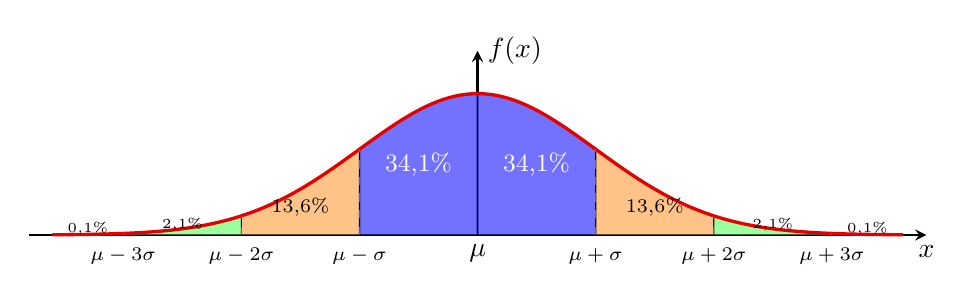
\begin{tikzpicture}[xscale=1.5, yscale=4.5]
    % Axes
    \draw[->, >=stealth, thick] (-3.8,0) -- (3.8,0) node[below] {$x$};
    \draw[->, >=stealth, thick] (0,0) -- (0,0.52) node[right] {$f(x)$};
    \node[below] at (0,0) {$\mu$};
    
    % Shaded regions
    % [-1, 1] 34.1% each
    \draw[fill=blue!65, opacity=0.85] (-1,0) -- plot[domain=-1:0, smooth, samples=50] (\x, {0.3989*exp(-0.5*\x*\x)}) -- (0,0) -- cycle;
    \draw[fill=blue!65, opacity=0.85] (0,0) -- plot[domain=0:1, smooth, samples=50] (\x, {0.3989*exp(-0.5*\x*\x)}) -- (1,0) -- cycle;
    
    % [-2, -1] and [1, 2] 13.6%
    \draw[fill=orange!55, opacity=0.85] (-2,0) -- plot[domain=-2:-1, smooth, samples=50] (\x, {0.3989*exp(-0.5*\x*\x)}) -- (-1,0) -- cycle;
    \draw[fill=orange!55, opacity=0.85] (1,0) -- plot[domain=1:2, smooth, samples=50] (\x, {0.3989*exp(-0.5*\x*\x)}) -- (2,0) -- cycle;

    % [-3, -2] and [2, 3] 2.1%
    \draw[fill=green!45, opacity=0.85] (-3,0) -- plot[domain=-3:-2, smooth, samples=50] (\x, {0.3989*exp(-0.5*\x*\x)}) -- (-2,0) -- cycle;
    \draw[fill=green!45, opacity=0.85] (2,0) -- plot[domain=2:3, smooth, samples=50] (\x, {0.3989*exp(-0.5*\x*\x)}) -- (3,0) -- cycle;

    % Curve
    \draw[domain=-3.6:3.6, smooth, samples=100, red!90!black, very thick] 
        plot (\x, {0.3989*exp(-0.5*\x*\x)});

    % Vertical dividers
    \foreach \x/\label in {-3/$\mu - 3\sigma$, -2/$\mu - 2\sigma$, -1/$\mu - \sigma$, 1/$\mu + \sigma$, 2/$\mu + 2\sigma$, 3/$\mu + 3\sigma$} {
        \draw[dashed, black!60] (\x, 0) -- (\x, {0.3989*exp(-0.5*\x*\x)});
        \node[below, font=\scriptsize] at (\x, -0.01) {\label};
    }

    % Percentage labels
    \node[white, font=\bfseries\small] at (-0.5, 0.2) {$34{,}1\%$};
    \node[white, font=\bfseries\small] at (0.5, 0.2) {$34{,}1\%$};
    \node[black, font=\scriptsize] at (-1.5, 0.08) {$13{,}6\%$};
    \node[black, font=\scriptsize] at (1.5, 0.08) {$13{,}6\%$};
    \node[black, font=\tiny] at (-2.5, 0.03) {$2{,}1\%$};
    \node[black, font=\tiny] at (2.5, 0.03) {$2{,}1\%$};
    \node[black, font=\tiny] at (-3.3, 0.018) {$0{,}1\%$};
    \node[black, font=\tiny] at (3.3, 0.018) {$0{,}1\%$};
\end{tikzpicture}
\end{center}

\begin{vidu}[VD 1]
Tốc độ chuyển dữ liệu từ máy chủ của ký túc xá đến máy tính của sinh viên vào buổi sáng chủ nhật có phân phối chuẩn với trung bình 60~Kbits/s và độ lệch chuẩn 4~Kbits/s. Xác suất để tốc độ chuyển dữ liệu lớn hơn 63~Kbits/s là:
\begin{enumerate}[label=\Alph*.]
    \item $0{,}2266$;
    \item $0{,}2144$;
    \item $0{,}1313$;
    \item $0{,}1060$.
\end{enumerate}

\paragraph{Giải.}
Gọi $X$ (Kbits/s) là tốc độ chuyển dữ liệu.

Theo giả thiết, ta có: $\mu = 60$, $\sigma = 4 \implies X \in N(60; 4^2)$.

Xác suất để tốc độ chuyển dữ liệu lớn hơn 63~Kbits/s là:
\begin{align*}
P(X > 63) &= P(63 < X < +\infty) \\
&= \varphi(+\infty) - \varphi\left(\frac{63 - 60}{4}\right) \\
&= 1 - \varphi(0{,}75).
\end{align*}
Tra bảng A4 với $z = 0{,}75$, ta được $\varphi(0{,}75) = 0{,}7734$.

Do đó:
\[
P(X > 63) = 1 - 0{,}7734 = 0{,}2266.
\]
Vậy đáp án đúng là \textbf{A}.
\end{vidu}

\begin{vidu}[VD 2]
Một kỳ thi đầu vào ở trường chuyên A quy định điểm đỗ là tổng số điểm các môn thi không được thấp hơn 15 điểm. Giả sử tổng điểm các môn thi của học sinh là biến ngẫu nhiên có phân phối chuẩn với trung bình 12 điểm. Biết rằng tỉ lệ học sinh thi đỗ là $25{,}14\%$. Độ lệch chuẩn là:
\begin{enumerate}[label=\Alph*.]
    \item 4 điểm;
    \item $4{,}5$ điểm;
    \item 5 điểm;
    \item $5{,}5$ điểm.
\end{enumerate}

\paragraph{Giải.}
Gọi $X$ là tổng điểm thi của học sinh. Theo giả thiết, $X \in N(12; \sigma^2)$.

Học sinh thi đỗ khi $X \ge 15$. Tỉ lệ học sinh thi đỗ là $25{,}14\% = 0{,}2514$, do đó:
\[
P(X \ge 15) = 0{,}2514.
\]
Mặt khác:
\[
P(X \ge 15) = 1 - \varphi\left(\frac{15 - 12}{\sigma}\right) = 1 - \varphi\left(\frac{3}{\sigma}\right).
\]
Suy ra:
\[
1 - \varphi\left(\frac{3}{\sigma}\right) = 0{,}2514 \iff \varphi\left(\frac{3}{\sigma}\right) = 1 - 0{,}2514 = 0{,}7486.
\]
Tra bảng A4 ngược lại, ta tìm được giá trị $z$ sao cho $\varphi(z) = 0{,}7486 \implies z = 0{,}67$.

Do đó:
\[
\frac{3}{\sigma} = 0{,}67 \implies \sigma = \frac{3}{0{,}67} \approx 4{,}4776 \approx 4{,}5 \text{ (điểm)}.
\]
Vậy đáp án đúng là \textbf{B}.
\end{vidu}

\begin{vidu}[VD 3]
Tuổi thọ của 1 loại máy lạnh A là BNN $X$ (năm) có phân phối $N(10; 6{,}25)$. Khi bán 1 máy lạnh A thì lãi được $1{,}4$ triệu đồng nhưng nếu máy lạnh phải bảo hành thì lỗ $1{,}8$ triệu đồng. Vậy để có tiền lãi trung bình khi bán mỗi máy lạnh loại này là $0{,}9$ triệu đồng thì cần phải quy định thời gian bảo hành là bao nhiêu?

\paragraph{Giải.}
Theo đề bài, tuổi thọ máy lạnh $X \sim N(10; 6{,}25)$, nghĩa là $\mu = 10$ và phương sai $\sigma^2 = 6{,}25 \implies \sigma = \sqrt{6{,}25} = 2{,}5$ (năm).

Gọi $t$ ($t > 0$, năm) là thời gian bảo hành cần quy định.

Máy lạnh phải bảo hành nếu tuổi thọ của nó không vượt quá $t$, tức là $X \le t$.

Xác suất (tỉ lệ) máy lạnh phải bảo hành là:
\[
p = P(X \le t) = \varphi\left(\frac{t - 10}{2{,}5}\right).
\]
Khi đó tỉ lệ máy lạnh không phải bảo hành là $1 - p$.

Gọi $Y$ (triệu đồng) là tiền lãi thu được khi bán 1 máy lạnh A. Bảng phân phối xác suất của $Y$ là:
\begin{center}
\renewcommand{\arraystretch}{1.3}
\begin{tabular}{|c|c|c|}
\hline
$Y$ & $-1{,}8$ & $1{,}4$ \\
\hline
$P$ & $p$ & $1 - p$ \\
\hline
\end{tabular}
\end{center}
Tiền lãi trung bình là:
\[
EY = -1{,}8 \times p + 1{,}4 \times (1 - p) = 1{,}4 - 3{,}2p.
\]
Để tiền lãi trung bình là $0{,}9$ triệu đồng:
\[
EY = 0{,}9 \iff 1{,}4 - 3{,}2p = 0{,}9 \iff 3{,}2p = 0{,}5 \iff p = \frac{0{,}5}{3{,}2} = 0{,}15625 \approx 0{,}1563.
\]
Ta có:
\[
P(X \le t) = 0{,}1563 \iff \varphi\left(\frac{t - 10}{2{,}5}\right) = 0{,}1563.
\]
Vì $0{,}1563 < 0{,}5$ nên theo tính chất đối xứng của hàm Laplace:
\[
\varphi\left(\frac{t - 10}{2{,}5}\right) = 1 - \varphi\left(-\frac{t - 10}{2{,}5}\right) = 0{,}1563 \implies \varphi\left(-\frac{t - 10}{2{,}5}\right) = 1 - 0{,}1563 = 0{,}8437.
\]
Tra bảng A4, ta thấy $\varphi(1{,}01) = 0{,}8438 \approx 0{,}8437$, suy ra:
\[
\varphi(-1{,}01) = 1 - 0{,}8438 = 0{,}1562 \approx 0{,}1563.
\]
Do đó:
\[
\frac{t - 10}{2{,}5} = -1{,}01 \iff t - 10 = -1{,}01 \times 2{,}5 = -2{,}525 \iff t = 10 - 2{,}525 = 7{,}475 \text{ (năm)}.
\]
Vậy cần quy định thời gian bảo hành là $7{,}475$ năm (tương đương khoảng 7 năm 5 tháng 21 ngày).
\end{vidu}

\vspace{1.5em}
\hrule
\vspace{1.5em}

\section{Một số quy luật phân phối liên tục khác (Tham khảo)}

\subsection{Phân phối Chi bình phương \texorpdfstring{$\chi^2(n)$}{Chi-binh-phuong}}

\begin{dinhnghia}
Nếu các biến ngẫu nhiên $X_1, X_2, \dots, X_n$ độc lập với nhau và đều có phân phối chuẩn tắc:
\[
X_i \in N(0; 1) \quad (i = 1, 2, \dots, n),
\]
thì biến ngẫu nhiên:
\[
X = \sum_{i=1}^n X_i^2 = X_1^2 + X_2^2 + \dots + X_n^2
\]
được gọi là có \textbf{phân phối Chi bình phương} với $n$ bậc tự do (degrees of freedom), ký hiệu là:
\[
X \in \chi^2(n) \quad \text{hay} \quad X \sim \chi^2(n).
\]

Hàm mật độ xác suất của $X \sim \chi^2(n)$ có dạng:
\[
f(x) = \begin{cases}
\dfrac{1}{2^{n/2} \Gamma\left(\dfrac{n}{2}\right)} e^{-x/2} x^{\frac{n}{2} - 1}, & x > 0 \\
0, & x \le 0.
\end{cases}
\]
Trong đó $\Gamma(p)$ là hàm Gamma Euler được định nghĩa bởi tích phân:
\[
\Gamma(p) = \int_0^{+\infty} e^{-x} x^{p - 1}\,dx \quad (p > 0).
\]
Các tính chất cơ bản của hàm Gamma:
\[
\Gamma(p + 1) = p \Gamma(p), \qquad \Gamma(1) = 1, \qquad \Gamma\left(\frac{1}{2}\right) = \sqrt{\pi}.
\]
(Đặc biệt, nếu $n \in \mathbb{N}^*$ thì $\Gamma(n) = (n - 1)!$).
\end{dinhnghia}

\begin{nhanxet}
Phân phối $\chi^2(n)$ do nhà thống kê học Karl Pearson đưa ra năm 1900. Đây là một trong những phân phối nền tảng của thống kê suy luận hiện đại, được ứng dụng rộng rãi trong bài toán ước lượng phương sai, kiểm định tính độc lập và kiểm định độ phù hợp chi-bình phương.
\end{nhanxet}

\subsection{Phân phối Student \texorpdfstring{$St(n)$}{Student}}

\begin{dinhnghia}
Nếu $T \sim N(0; 1)$ và $Y \sim \chi^2(n)$ là hai biến ngẫu nhiên độc lập với nhau, thì biến ngẫu nhiên:
\[
X = T \sqrt{\frac{n}{Y}} = \frac{T}{\sqrt{\dfrac{Y}{n}}}
\]
được gọi là có \textbf{phân phối Student} với $n$ bậc tự do, ký hiệu là:
\[
X \in St(n) \quad \text{hay} \quad X \sim t(n).
\]

Hàm mật độ xác suất của $X \sim St(n)$ có dạng:
\[
f(x) = \frac{\Gamma\left(\dfrac{n + 1}{2}\right)}{\sqrt{n\pi} \, \Gamma\left(\dfrac{n}{2}\right)} \left(1 + \frac{x^2}{n}\right)^{-\frac{n + 1}{2}}, \quad x \in \mathbb{R}.
\]
\end{dinhnghia}

\begin{nhanxet}
Phân phối Student do William Sealy Gosset đưa ra năm 1908 (dưới bút danh ``Student'' khi ông đang làm việc tại nhà máy bia Guinness). Đồ thị hàm mật độ của phân phối Student đối xứng hình chuông qua trục tung tương tự như phân phối chuẩn tắc, nhưng có phần đuôi dày hơn (xác suất các giá trị xa tâm lớn hơn). Khi số bậc tự do $n \to \infty$, phân phối Student tiệm cận phân phối chuẩn tắc $N(0; 1)$.
\end{nhanxet}

\vspace{1.5em}
\hrule
\vspace{1.5em}

\section{Bài tập vận dụng}

\begin{enumerate}[label=\textbf{\arabic*.}]
    \item Một máy tính có 20 thư mục, trong đó có 5 thư mục bị nhiễm virus. Chọn ngẫu nhiên 6 thư mục để kiểm tra xem có bị nhiễm virus hay không.
    \begin{enumerate}[label=\alph*)]
        \item Tính xác suất có ít nhất 3 thư mục bị nhiễm virus.
        \item Trung bình có bao nhiêu thư mục bị nhiễm trong 6 thư mục được chọn?
    \end{enumerate}

    \item Một kĩ thuật viên theo dõi 12 máy tự động. Xác suất để mỗi máy cần đến sự điều chỉnh của kĩ thuật viên trong mỗi ngày là $0{,}1$. Các máy này hoạt động độc lập nhau.
    \begin{enumerate}[label=\alph*)]
        \item Gọi $X$ là số máy cần sự điều chỉnh mỗi ngày. Tìm phân phối xác suất của $X$.
        \item Tìm xác suất mỗi ngày có ít nhất 1 máy cần điều chỉnh.
    \end{enumerate}

    \item Xác suất trúng mỗi tờ vé số là $0{,}001$.
    \begin{enumerate}[label=\alph*)]
        \item Hỏi nếu mua 20 tờ vé số thì xác suất trúng 2 tờ là bao nhiêu?
        \item Hỏi trung bình mua 20 tờ vé số thì trúng bao nhiêu tờ?
    \end{enumerate}

    \item Có một trò chơi điện tử được phát hành. $60\%$ người chơi hoàn thành được hết các level và có $30\%$ trong số đó sau đó mua phiên bản tiếp theo.
    \begin{enumerate}[label=\alph*)]
        \item Hỏi trung bình trong 15 người chơi, có bao nhiêu người mua phiên bản tiếp theo?
        \item Xác suất có ít nhất 2 người chơi sẽ mua phiên bản mới trong 15 người chơi?
    \end{enumerate}

    \item Trung bình 5 phút có 15 người vào một đại lý bưu điện. Tính xác suất trong 1 phút có 4 người vào đại lý bưu điện đó. Biết rằng số người vào đại lý là một ĐLNN rời rạc có phân phối Poisson.

    \item Một công ty cung cấp dịch vụ internet có trung bình 20 khách hàng đăng kí tài khoản mới mỗi ngày. Biết rằng số tài khoản mới đăng kí mỗi ngày có phân phối Poisson.
    \begin{enumerate}[label=\alph*)]
        \item Tính xác suất có ít nhất 3 tài khoản mới đăng kí trong ngày mai.
        \item Tính xác suất có ít nhất 6 tài khoản mới đăng kí trong 2 ngày tới.
    \end{enumerate}

    \item Nếu chiều cao $X$ của sinh viên nam có phân phối chuẩn với trung bình $166\text{ cm}$, độ lệch chuẩn $4\text{ cm}$, thì có bao nhiêu $\%$ sinh viên nam có chiều cao:
    \begin{enumerate}[label=(\arabic*)]
        \item Từ $162\text{ cm}$ đến $170\text{ cm}$;
        \item Từ $154\text{ cm}$ đến $178\text{ cm}$;
        \item Trên $180\text{ cm}$;
        \item Dưới $160\text{ cm}$.
    \end{enumerate}

    \item Giả sử đường kính trong của các vòng đệm cao su do một máy sản xuất có phân phối chuẩn, với đường kính trong trung bình là $1{,}27\text{ cm}$ và độ lệch chuẩn là $0{,}01\text{ cm}$. Đường kính trong của các vòng đệm này được phép có dung sai từ $1{,}25\text{ cm}$ đến $1{,}29\text{ cm}$, ngược lại thì các vòng đệm được xem bị hỏng. Hãy xác định tỷ lệ phần trăm các vòng đệm do máy này sản xuất bị hỏng.

    \item Cho BNN $X$ có phân phối chuẩn với $EX = 10$ và $P(10 < X < 20) = 0{,}3$. Tính $P(0 < X \le 15)$?

    \item Giả sử thời gian khách phải chờ để được phục vụ tại một cửa hàng là BNN $X$ (phút), $X \in N(4{,}5; 1{,}21)$.
    \begin{enumerate}[label=\arabic*)]
        \item Tính xác suất khách phải chờ từ $3{,}5$ phút đến 5 phút.
        \item Tính thời gian tối thiểu $t$ nếu xác suất khách phải chờ vượt quá $t$ là không quá $5\%$.
    \end{enumerate}

    \item Tuổi thọ $X$ (năm) của một loại bóng đèn $A$ là BNN tuân theo luật phân phối chuẩn $N(4; 2{,}25)$.
    \begin{enumerate}[label=\alph*.]
        \item Tính tỉ lệ bóng đèn $A$ có tuổi thọ từ $4{,}5$ năm trở lên.
        \item Quan sát ngẫu nhiên 1 bóng đèn loại $A$ thấy nó có tuổi thọ trên tuổi thọ trung bình. Hãy tính xác suất bóng đèn đó có tuổi thọ không quá 5 năm.
        \item Cần mua bao nhiêu bóng đèn loại $A$ để xác suất mua được ít nhất 1 bóng có tuổi thọ từ 6 năm trở lên không nhỏ hơn $90\%$?
    \end{enumerate}

    \item Đường kính của một loại trục máy do máy tiện làm ra là một đại lượng ngẫu nhiên có phân phối chuẩn, với giá trị trung bình là $25\text{ mm}$, và phương sai là $44{,}1\text{ mm}^2$. Trục máy được xem là đạt tiêu chuẩn kỹ thuật nếu đường kính nằm trong khoảng từ $23{,}44\text{ mm}$ đến $26{,}56\text{ mm}$.
    \begin{enumerate}[label=\arabic*)]
        \item Tìm tỉ lệ trục máy đạt tiêu chuẩn kỹ thuật.
        \item Phải sản xuất ít nhất bao nhiêu trục để khả năng có ít nhất 1 trục đạt tiêu chuẩn kỹ thuật không dưới $99{,}73\%$?
        \item Tính tỉ lệ trục máy đạt tiêu chuẩn kỹ thuật trong số các trục máy có đường kính trên $25\text{ mm}$.
    \end{enumerate}
\end{enumerate}
